\documentclass{article} % For LaTeX2e
\usepackage{iclr2026_conference}

\input{math_commands.tex}

\usepackage{hyperref}
\usepackage{url}
\usepackage{booktabs}
\usepackage{graphicx}
\usepackage{amsmath}
% The template's `times` package silently falls back to Latin Modern under
% tectonic; newtx is the same Times look with matching math (subsumes amssymb).
\usepackage{newtxtext,newtxmath}
\usepackage{multirow}
\usepackage{subcaption}

% De-anonymized draft; comment out for double-blind submission.
\iclrfinalcopy

\newcommand{\gap}{\mathrm{gap}}
\newcommand{\Floor}{\mathrm{Floor}}
\newcommand{\reenc}{\mathrm{reenc}}
\newcommand{\sigmastar}{\sigma^{\!*}}

% \textit (not \emph): the style sets the title in small caps, where \emph's
% shape toggle is silently substituted away.
\title{\textit{Almost} Equivalent: Measuring When Downscaled\\
Images Carry the Flow-Matching Training Signal}

\author{Seunghyun Ji\\
Independent researcher\\
\texttt{standingbehindnv@gmail.com}
}

\begin{document}

\maketitle
% Drop the "Published as a conference paper at ICLR 2026" running head
% (set by \maketitle under \iclrfinalcopy) for this draft.
\fancyhead{}
\renewcommand{\headrulewidth}{0pt}

\begin{abstract}
Scale-wise diffusion schemes rest on a spectral argument: flow-matching
noising progressively masks high spatial frequencies, so above some noise
level a downscaled latent carries \emph{almost} the full surviving signal.
We ask whether this licenses a training-side substitution --- can the
gradient of a low-rank adapter be computed from a downscaled latent at high
noise without changing what is learned?
We measure per-noise-level gradient agreement between native and downscaled
latents on a DiT-based flow-matching model, with a fresh-noise floor and a
VAE re-encoding control, and find that the spectral account fails
quantitatively at the gradient level: the measured safety crossover sits at
$\sigma\!\approx\!0.5$, $3.5\times$ above the spectral prediction, and a
$2\times$ downscale is never gradient-safe at any noise level --- a gap of
$0.3$ persists even at $\sigma=0.94$, where the input is $97\%$ noise by
power. The reason is structural: expected gradients average noise out
rather than being masked by it, and the flow-matching target $v=\epsilon-x$
carries the clean image at unit amplitude at every $\sigma$.
The gap decomposes into two mechanistically distinct terms: a
noise-dependent input term whose amplitude is governed by the
\emph{downscale ratio}, and a $\sigma$-independent floor governed by the
\emph{absolute token count} of the downscaled grid, concentrated in early
blocks, and further separable --- by a positional-interpolation
intervention --- into a rotary-position-embedding share and an irreducible
graph residue.
The practical output is a measured $(\text{route},\sigma)$ safety map and
an opt-in $\sigma$-conditional trainer that draws the noise level first and
substitutes the downscaled latent only on measured-safe steps, for a
${\sim}14\%$ wall-clock reduction at fixed step count on our corpus.
\end{abstract}

\section{Introduction}
\label{sec:intro}

The cost of a diffusion-transformer forward pass grows superlinearly with
resolution: token count grows quadratically with edge length, and attention
cost grows again in token count. A family of recent methods therefore runs
part of the computation at reduced resolution, justified by a spectral
observation about the forward noising process: under flow-matching noising
$z_\sigma = (1-\sigma)x + \sigma\epsilon$, the per-frequency
signal-to-noise ratio falls with $\sigma$, and high spatial frequencies
drop below the noise floor first. Above a crossover noise level, a
downscaled latent is claimed to carry \emph{almost} the full surviving
signal --- the premise behind scale-wise distillation
\citep{starodubcev2025swd}, pyramidal flow matching \citep{jin2024pyramidal},
and progressive-resolution training schedules more broadly
\citep{karras2018progressive,chen2024pixartalpha,hoogeboom2023simple}.

These methods change the \emph{inference} trajectory or the model itself.
We ask a narrower, training-side question: at high noise, can the
\emph{gradient} of an adapter be computed on a downscaled latent as a
drop-in substitute for the native one --- same model, same objective, same
$\sigma$ distribution, only the spatial grid changed on some steps? If the
spectral account governed, the answer would be yes above the spectral
crossover $\sigmastar\!\approx\!0.14$ for our latents, and the payoff would
be large: on our corpus roughly half of all training draws sit at
$\sigma>0.5$.

We test this directly. Our instrument computes, per noise-level bin, the
cosine between adapter gradients from native and downscaled latents,
calibrated by a fresh-noise floor (how much two native gradient estimates
disagree anyway) and a VAE re-encoding control (the cost of a decode--encode
round trip with no resolution change). The headline results:

\begin{enumerate}
\item \textbf{The spectral prediction fails at the gradient level}
(\S\ref{sec:phase0}). The measured crossover for the mildest downscale
($0.875\times$ edge) is $\sigma\!\approx\!0.5$, not the closed-form
spectral prediction $0.136$; a $2\times$ downscale never becomes safe at
any $\sigma$, retaining a gap of ${\sim}0.3$ at $\sigma=0.94$ where the
input is essentially pure noise. Spectral sufficiency of the \emph{input}
licenses representability, not gradient equivalence --- and we argue the
divergence is structural, not incidental: the trained quantity
$\mathbb{E}_\epsilon[\nabla_\theta \mathcal{L}]$ averages noise out rather
than being masked by it, and the flow-matching target $v=\epsilon-x$
carries the clean image at coefficient one at every $\sigma$
(\S\ref{sec:whyfail}).
\item \textbf{The gap has a two-term anatomy} (\S\ref{sec:anatomy}):
$\gap_e(\sigma) \approx A_e\, m(\sigma)/G(\sigma)^p + \Floor_e$.
The residual-mismatch shape $m(\sigma)$ is \emph{route-uniform} --- all
route identity lives in the network's input-output Jacobian, not in the
prediction error. The input-term amplitude $A_e$ is governed by the
downscale \emph{ratio} (an iso-severity probe at $1.6\times$ different
absolute size reproduces the same curve), while the $\sigma$-independent
floor $\Floor_e$ is governed by \emph{absolute target token count},
concentrates in early blocks, and decomposes --- via an exact
positional-interpolation intervention on the rotary embedding --- into a
coordinate-system share $\mathrm{RoPE}_e$ (most of the mild-route floor)
and a non-positional graph residue $\mathrm{Resid}_e$ (the bulk of the
harsh-route floor). The positional share is removable only in the
noise-dominated regime; with image content in the input, the stretched
coordinates are off-manifold and \emph{add} error, so it is a mechanism
finding, not a training lever.
\item \textbf{A measured safety map and a practical trainer}
(\S\ref{sec:map}--\ref{sec:trainer}). Safety is a per-route boundary
$\sigmastar(\text{route})$, not a universal ratio rule:
$\{1024{\to}896$ at $\sigma>0.5$; $1280{\to}1024$ at
$\sigma \gtrsim 0.75\}$, while $896{\to}768$ and every ${\to}512$ route are
never safe. We wire the measured-safe route into an opt-in
$\sigma$-conditional trainer --- draw $\sigma$ first, fetch the downscaled
latent only when the whole batch is above the gate --- for a ${\sim}14\%$
wall-clock reduction at a fixed step budget, with a $\sigma$-gated
banded rotary alignment as a measured refinement.
\end{enumerate}

Everything here is deliberately observational-first: verdict criteria were
frozen before each probe ran, and each mechanistic claim is grounded in a
designated falsification test (several of which fired and killed proposed
routes; we report those too).

\section{Related work}
\label{sec:related}

\paragraph{Scale-wise and progressive-resolution diffusion.}
Progressive growing \citep{karras2018progressive} and resolution curricula
\citep{chen2024pixartalpha,hoogeboom2023simple} train at increasing
resolution as a schedule. Pyramidal flow matching \citep{jin2024pyramidal}
and scale-wise distillation (SwD) \citep{starodubcev2025swd} tie resolution
to the noise level itself, with SwD giving the spectral analysis we take as
the hypothesis under test: their Fig.~1-style argument shows the noised
downscaled latent is close in distribution to a downscaled noised latent
above a crossover $\sigma$. Our contribution is orthogonal to all of these:
we measure whether that input-level closeness transfers to the
\emph{training gradient}, holding model and objective fixed --- and find it
does not transfer at the predicted scale.

\paragraph{Flow matching and DiT.}
We work in the flow-matching / rectified-flow formulation
\citep{lipman2023flow,liu2023rectified,esser2024scaling} on a Diffusion
Transformer \citep{peebles2023dit} with rotary position embeddings
\citep{su2024roformer}. Adapters are LoRA \citep{hu2022lora}.

\paragraph{Positional extension.}
Position interpolation \citep{chen2023pi}, banded/frequency-selective
variants (YaRN, \citealp{peng2024yarn}), and diffusion-specific dynamic
position extrapolation \citep{issachar2025dype,zhao2026sigma} rescale
rotary coordinates to evaluate a model at unseen grid sizes. We use exact
positional interpolation as a \emph{causal intervention} --- matching the
downscaled grid's relative phase geometry to native --- to decompose the
resolution-sensitivity floor, and adopt the $\sigma$-gated band schedule of
\citet{zhao2026sigma} (functional form only; their spectral scale laws
mispredict our measured boundaries, consistent with our main finding) as a
training-time refinement.

\paragraph{Gradient-agreement methodology.}
Reading training decisions off gradient cosines against a
noise-redraw floor follows the general logic of gradient-noise-scale
analyses \citep{mccandlish2018gns}; our estimator operates per
$\sigma$-bin with means over images, the regime we found reliable
(split-half reliability $0.73$--$0.88$), rather than per-image rankings,
which were pure noise in our earlier attempts.

\section{Setup and instrument}
\label{sec:setup}

\paragraph{Model and data.}
All measurements use Anima, an open DiT-based flow-matching text-to-image
model (28 transformer blocks, 3D rotary position embeddings, Qwen-family
VAE), fine-tuned with LoRA adapters on an illustration corpus. Images are
bucketed by native aspect ratio into resolution \emph{tiers} indexed by
nominal edge length $e \in \{512, 768, 896, 1024, 1280\}$; a tier-$e$ image
occupies roughly $(e/16)^2$ latent-patch tokens (e.g.\ ${\sim}4{,}100$
tokens at 1024, ${\sim}3{,}000$ at 896, ${\sim}2{,}160$ at 768,
${\sim}1{,}000$ at 512). The probe adapter is a LoRA soup checkpoint
trained at native tiers; we return to this operating-point caveat in
\S\ref{sec:limitations}.

\paragraph{Objective and noising.}
With clean latent $x$, noise $\epsilon \sim \mathcal{N}(0, I)$, and
$\sigma \in (0,1]$, the noised input is
$z_\sigma = (1-\sigma)\,x + \sigma\,\epsilon$ and the flow-matching target
is $v = \epsilon - x$; the loss is
$\|\hat v_\theta(z_\sigma, \sigma, c) - v\|^2$ with gradients taken with
respect to adapter parameters only.

\paragraph{Demotion.}
A \emph{demotion} $e_{\mathrm{nat}} {\to} e$ replaces the native latent
with one produced by pixel-space downscaling of the source image to the
tier-$e$ bucket followed by VAE re-encoding --- the ordering SwD validated
(``strategy~B''); we never downsample in latent space. The caption, the
noise draw structure, and the $\sigma$ under test are held fixed; only the
spatial grid changes.

\paragraph{The gradient probe.}
For each image and each of $B$ uniform $\sigma$-bins we accumulate adapter
gradients over $D$ stratified noise draws per arm (shipped runs:
$8 \times 8$ unless noted; $N = 40$ images) and compare arms by cosine
similarity of the flattened accumulated gradients:
\begin{itemize}
\item \textbf{floor}: two independent draw sets at native resolution ---
the ``how much do gradients differ anyway'' null;
\item \textbf{reenc}: decode--re-encode at native resolution --- isolates
the VAE round-trip cost that demotion necessarily pays;
\item \textbf{demote arms}: one per edge $e$ under test.
\end{itemize}
The verdict quantity is the \emph{demotion gap}
\begin{equation}
\gap_e(\sigma) \;=\; \cos_{\mathrm{floor}}(\sigma) \;-\;
\cos\!\big(g_{\mathrm{nat}}(\sigma),\, g_{e}(\sigma)\big),
\end{equation}
in cosine units (a mismatch \emph{fraction}, scale-free; bin-mean SEM
${\sim}0.02$ at $N{=}40$). Gap subtraction, not absolute cosines, is the
valid read: the floor itself moves with $\|g\|$ across bins. The
re-encoding control $\gap_\reenc \approx 0$ (band $\pm 0.04$) is the
instrument-validity witness in every run, and every bin-mean curve must
pass a split-half reliability check over images --- a discipline forced on
us by an earlier failure in which per-image rankings from the same
gradients had split-half reliability indistinguishable from zero.
Uniform $\sigma$-bins make the training-time $\sigma$-density irrelevant
to the map; density-weighting the bins reproduces our earlier pooled
(marginalized) measurements as a consistency check.

\section{The spectral prediction fails at the gradient level}
\label{sec:phase0}

\begin{figure}[t]
\centering
\begin{subfigure}[t]{0.495\textwidth}
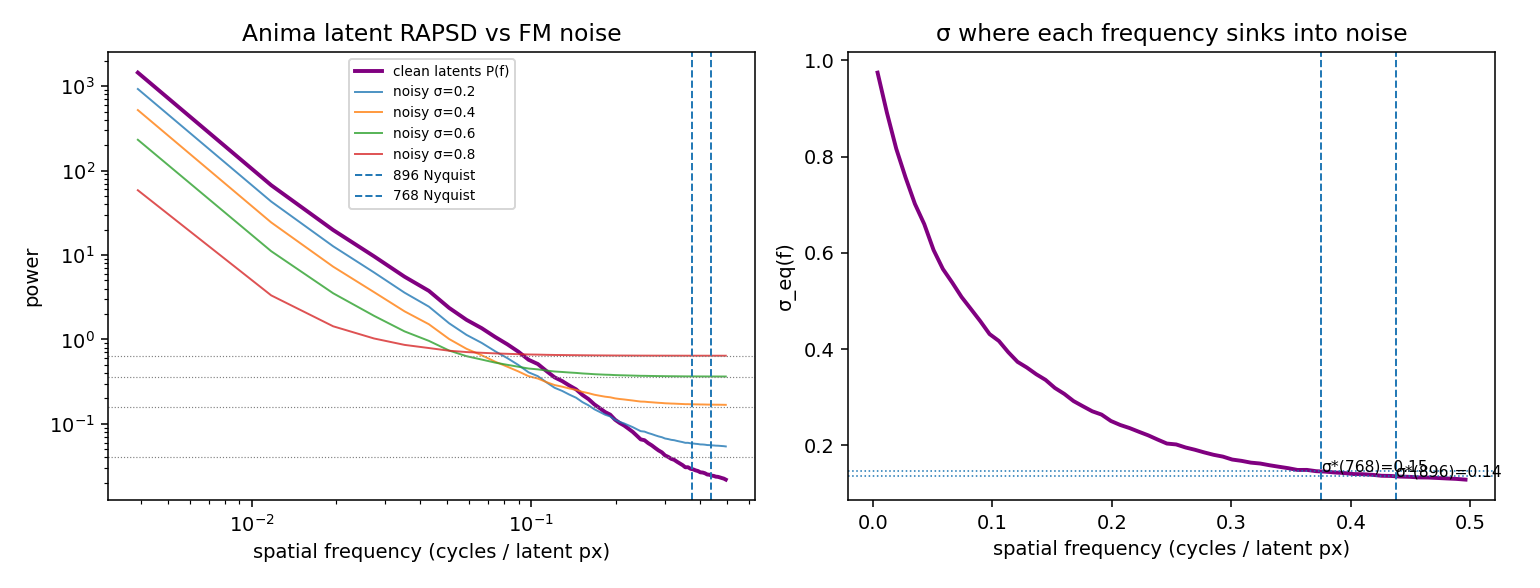
\includegraphics[width=\linewidth]{figs/rapsd.png}
\caption{Latent RAPSD and closed-form crossover
$\sigma_{\mathrm{eq}}(f)$. Predicted $\sigmastar$: $0.136$ / $0.146$ /
${\sim}0.20$ for demotion to 896 / 768 / 512.}
\label{fig:rapsd}
\end{subfigure}\hfill
\begin{subfigure}[t]{0.495\textwidth}
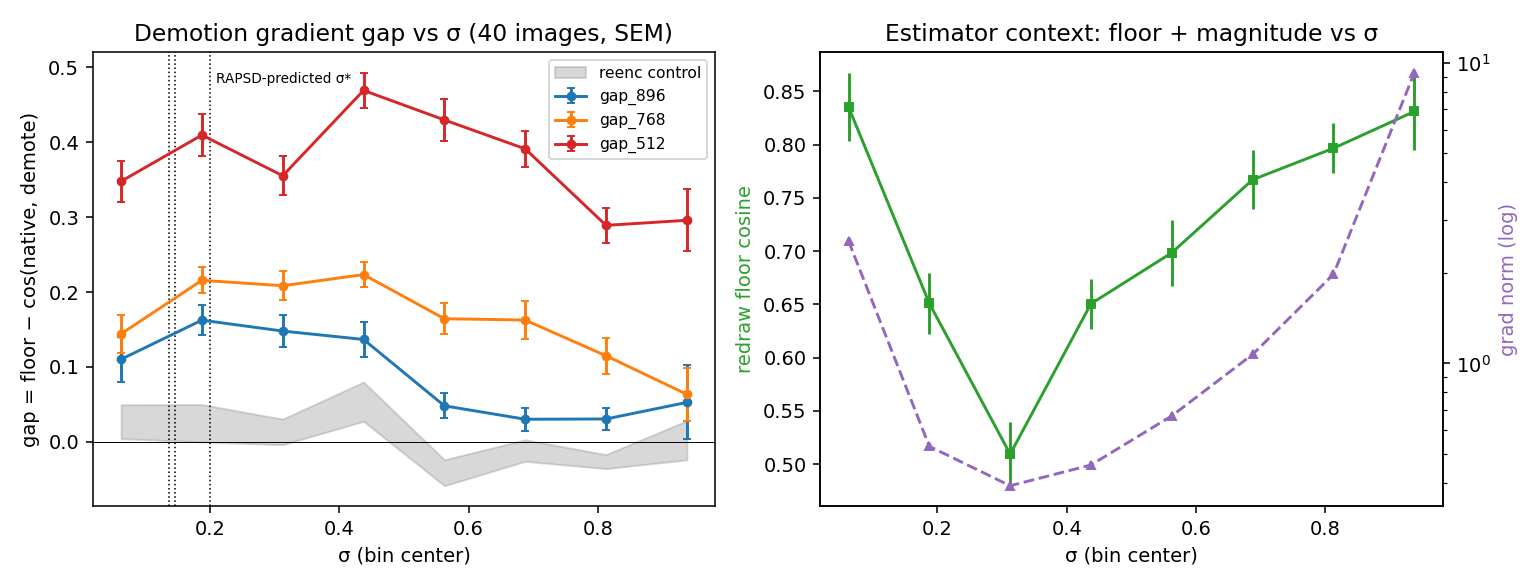
\includegraphics[width=\linewidth]{figs/gap_vs_sigma.png}
\caption{Measured demotion gap per $\sigma$-bin ($1024$-tier natives,
$N{=}40$). The 896 route floors at $\sigma\!\approx\!0.5$; 512 never
floors.}
\label{fig:gapcurves}
\end{subfigure}
\caption{The spectral prediction (left) versus the gradient measurement
(right). The crossover is off by ${\sim}3.5\times$ and the $2\times$
downscale never becomes safe.}
\label{fig:phase0}
\end{figure}

\paragraph{The prediction.}
Under unit-variance white noise the per-frequency crossover has the closed
form $\sigma_{\mathrm{eq}}(f) = \sqrt{P(f)}\,/\,(1+\sqrt{P(f)})$, where
$P$ is the clean-latent radially averaged power spectral density. Anima's
VAE latents are high-frequency-quiet ($P(f) < 1$ above $f \approx 0.16$
cycles/latent-pixel; latent variance $0.42$), giving
$\sigmastar(896) = 0.136$, $\sigmastar(768) = 0.146$,
$\sigmastar(512) \approx 0.20$, with tight per-image spread
(p10--p90 ${\approx}\,0.11$--$0.16$): the spectral crossover is
image-generic, and if it governed, demotion would be safe over almost the
entire $\sigma$ axis (Fig.~\ref{fig:rapsd}).

\paragraph{The measurement.}
Table~\ref{tab:phase0} gives the measured gap curves for $1024$-tier
natives demoted to $896/768/512$.

\begin{table}[t]
\caption{Demotion gap by $\sigma$-bin, $1024$-tier natives ($N{=}40$,
bin-mean SEM ${\sim}0.02$, re-encoding control $|\gap_\reenc| \le 0.054$
everywhere, split-half reliability $0.73$--$0.83$). Bold = within the
re-encoding band. The spectral account predicts collapse above the second
bin for every route.}
\label{tab:phase0}
\centering
\small
\begin{tabular}{lcccccccc}
\toprule
$\sigma$ bin center & 0.06 & 0.19 & 0.31 & 0.44 & 0.56 & 0.69 & 0.81 & 0.94 \\
\midrule
$\gap_{896}$ (ratio $0.875$) & .110 & .162 & .148 & .137 & \textbf{.048} & \textbf{.030} & \textbf{.030} & .053 \\
$\gap_{768}$ (ratio $0.75$)  & .144 & .216 & .208 & .223 & .164 & .163 & .115 & .063 \\
$\gap_{512}$ (ratio $0.5$)   & .348 & .410 & .355 & .469 & .430 & .391 & .289 & .296 \\
\midrule
$\cos_{\mathrm{floor}}$ & .84 & .65 & .51 & .65 & .70 & .77 & .80 & .83 \\
$\|g\|$ (native) & 2.6 & 0.5 & 0.4 & 0.5 & 0.7 & 1.1 & 2.0 & 9.3 \\
\bottomrule
\end{tabular}
\end{table}

Three reads, against criteria frozen before the run:
(i)~$\sigma$-dependence is real and in the predicted direction
(Spearman $\sigma{\to}\gap$: $-0.69/-0.57/-0.36$), and tier ordering holds
at every bin --- the \emph{qualitative} spectral intuition survives;
(ii)~the crossover for the mildest route is $\sigma \approx 0.5$, not
$0.136$ --- off by ${\sim}3.5\times$;
(iii)~the $2\times$ downscale route retains $\gap \approx 0.3$ at
$\sigma = 0.94$, where the input is ${\sim}97\%$ noise by power in every
band the coarse grid cannot represent. There is no noise level at which a
$2\times$-downscaled latent yields the native gradient.

\paragraph{Ratio does not transfer.}
Re-running the probe one tier down ($896$-tier natives, demote to
$768/512$) fails its pre-registered bar: $896{\to}768$ (ratio $0.857$,
nearly identical to the passing $0.875$) retains a high-$\sigma$ residual
of $0.06$--$0.12$, roughly $2\times$ the $1024{\to}896$ plateau and
outside the re-encoding band, while the two-tiers-down control stays
elevated everywhere. ``One tier down at high $\sigma$'' is \emph{not} the
invariant; \S\ref{sec:anatomy} shows why (the floor is governed by
absolute size, and $896{\to}768$'s floor alone exceeds the band).

\subsection{Why the spectral account must fail here}
\label{sec:whyfail}

The failure is structural, not a peculiarity of our model. Two
observations, neither of which involves the spectrum of $z_\sigma$:

\textbf{(a) Expected gradients are never noise-masked.} ``Noise power
exceeds signal power in band $f$'' is a statement about a single sample of
$z_\sigma$. The quantity training consumes is
$\mathbb{E}_\epsilon[\nabla_\theta \mathcal{L}]$ --- an expectation that
averages the noise out and retains attenuated signal at \emph{any} SNR.
Input-level sufficiency licenses inference-time substitution; it never
licenses training-dynamics equivalence.

\textbf{(b) The target carries the clean image at unit amplitude at every
$\sigma$.} The flow-matching target is $v = \epsilon - x$. The
\emph{input} is progressively noise-masked as $\sigma \to 1$, but $x$ sits
in the \emph{target} at coefficient one even at $\sigma = 0.94$. Writing
the adapter gradient as $g = J^{\!\top} r$ (Jacobian times residual), the
two grids can disagree through $J$ itself --- attention softmax over a
different token count $N$, rotary phase density, sequence-length-dependent
normalization --- regardless of how little image signal the input retains.

Both observations predict exactly what we measure at $\sigma = 0.94$: a
route-ordered gap that survives an input of essentially pure noise. The
next section pins this down experimentally.

\section{Anatomy of the gap: a two-term account}
\label{sec:anatomy}

We propose, and then test term by term, the decomposition
\begin{equation}
\gap_e(\sigma) \;\approx\;
\underbrace{A_e \cdot m(\sigma)\,/\,G(\sigma)^{p}}_{\text{input branch }S_1}
\;+\; \underbrace{\Floor_e}_{\text{graph term}},
\qquad p \in [1,2],
\label{eq:twoterm}
\end{equation}
where $m(\sigma)$ is the (route-uniform) mismatch of the model's mean
prediction residual across grids, $G(\sigma) = \|g\|$ is the total
gradient scale (the cosine's implicit denominator), $A_e$ is a
$\sigma$-independent route amplitude, and $\Floor_e$ is a
$\sigma$-independent term carried by the network function itself. The
formula is structural rather than a quantitative fit: $p$ is fixed only to
$[1,2]$ by cosine geometry ($2$ in the small-orthogonal-mismatch limit),
and $A_e$ absorbs units. Its value is that each object is independently
measurable, and that it retrodicts every curve shape and route ordering we
observe. The account was pre-registered with an outcome matrix (including
a kill switch) before the discriminating runs; it survived, and
subsequently absorbed four refinements, each from a designated probe.

\subsection{The floor exists, is $\sigma$-independent, and is not carried
by the input}
\label{sec:floor}

\begin{table}[t]
\caption{Isolating the floor. \textbf{Endpoint}: at $\sigma{=}1$ the input
is exactly $\epsilon$, so any gap \emph{is} the floor by construction
($16$ draws). \textbf{x-zero}: the image is zeroed in both input and
target on every grid; any surviving gap is pure graph-shape sensitivity.
Pre-registered bands in brackets; all pass, and the account's kill switch
(all endpoint gaps ${\approx}\,0$) does not fire.}
\label{tab:floor}
\centering
\small
\begin{tabular}{lcccc}
\toprule
route & endpoint gap @ $\sigma{=}1$ (SEM) & band & x-zero @ $\sigma{=}1$ (SEM) \\
\midrule
re-encoding control & $-0.038$ (.032) & $[-.04, .04]$ & --- \\
$1024{\to}896$ & $-0.009$ (.042) & $[0, 0.08]$ & $0.004$ (.018) \\
$1024{\to}768$ & $+0.127$ (.054) & $[0.04, 0.15]$ & $0.064$ (.028) \\
$1024{\to}512$ & $+0.326$ (.059) & $[0.2, 0.4]$ & $0.299$ (.040) \\
\bottomrule
\end{tabular}
\end{table}

Two designated probes (Table~\ref{tab:floor}) establish the graph term.
At the $\sigma = 1$ \emph{endpoint} the input is pure $\epsilon$ ---
identical in distribution across arms --- so the input-information term is
zero by construction, and the measured gaps ($\approx\!0$ / $0.13$ / $0.33$
for $896/768/512$) match the high-$\sigma$ plateaus of
Table~\ref{tab:phase0}: the plateau \emph{is} the floor. The \emph{x-zero}
probe removes the image from input \emph{and} target everywhere; for the
$2\times$ route the surviving gap equals the endpoint gap ($0.30$ vs
$0.33$) --- the floor is essentially all network-function term, with
per-image content contributing nothing. Two further exonerations: the
re-encoding control sits in band (the VAE round trip is not the cause),
and a forward-only probe of the model's caption-conditioned \emph{prior}
across grids shows route distances that are flat where the floors are
strongly ordered --- so the floor's route-ordering lives in the Jacobian
factor $J$, not in the model's resolution-conditioned prior $\hat
x_{\mathrm{prior}}$, and not in a training-distribution discontinuity (the
never-trained 1280 grid is no more distant from 1024 than heavily-trained
adjacent pairs are from each other).

\subsection{The input branch: a route-uniform numerator over a U-shaped
denominator}
\label{sec:inputbranch}

\paragraph{$m(\sigma)$ is universal.}
Measuring the mean prediction residual
$\bar r = \mathbb{E}_\epsilon[\hat v - (\epsilon - x)]$ per grid and
$\sigma$ --- the exact $r$ in $g = J^{\!\top} r$ --- shows a strong,
monotone $\sigma$-shape (cross-grid excess $0.89 \to 0.36$ in relative
$L_2$ from $\sigma{=}0.125$ to $1$) that is the \emph{same for every
route} within $\pm 0.02$, across routes whose gradient floors span $0$ to
$0.3$ and whose crossovers span $0.5$ to nonexistent. All route identity
therefore lives in $J$, not in the prediction error --- a pre-registered
null that would have falsified the account had the residual curves been
route-ordered. The decay is smooth, Wiener-like posterior shrinkage with
no hard gate at the spectral crossover: gap curves read as ``collapsed''
where $S_1$ sinks below the instrument band, not at
$\sigma_{\mathrm{eq}}$.

\paragraph{$G(\sigma)$ shapes the curve.}
Because the gap is a cosine it measures a mismatch \emph{fraction}; the
total gradient norm is U-shaped in $\sigma$ ($2.6 \to 0.4$ at
$\sigma\!\approx\!0.3 \to 9.3$; Table~\ref{tab:phase0}, last row) --- large
at high $\sigma$ where the model is pulling composition out of the prior
and the residual is image-scale, small in the mid-$\sigma$ refinement
regime, and inflated again at low $\sigma$ by irreducible $\epsilon$.
A monotone absolute mismatch divided by a U-shaped norm yields exactly the
measured interior-peaked gap curves: bin-mean gap tracks $1/\|g\|$
(Spearman $+0.55$ to $+0.90$ across arms and runs, and within images), and
renormalizing by $G$ flips the anomalous low-$\sigma$ dip into the
monotone maximum in every arm of both runs. This is a post-hoc
consistency analysis (flagged as such): it explains the \emph{shape}; all
safety criteria stay in cosine units, since direction is what a
normalized optimizer consumes.

\subsection{The governors: ratio sets the amplitude, absolute size sets
the floor}
\label{sec:governors}

\begin{table}[t]
\caption{Iso-severity probe: gap by $\sigma$-bin on the $1280$-tier cache
($N{=}24$, $4$ draws/bin) against the corpus $1024{\to}896$ curve. The
ratio-matched routes coincide within ${\sim}1.4$ combined SEM at every bin
despite a $1.6\times$ difference in absolute target size; the same-native
harsher-ratio route separates. $^{*}$$896$'s canonical $16$-draw endpoint
is $-0.009$ (Table~\ref{tab:floor}).}
\label{tab:isoseverity}
\centering
\small
\begin{tabular}{lccccc}
\toprule
$\sigma$ & 0.125 & 0.375 & 0.625 & 0.875 & 1.0 \\
\midrule
re-encoding control & $+.047$ & $-.005$ & $+.048$ & $+.020$ & $-.012$ \\
$1280{\to}1120$ (ratio $.875$) & .129 & .110 & .054 & $-.012$ & $-.007$ \\
$1280{\to}1024$ (ratio $.80$)  & .170 & .178 & .111 & .002 & .061 \\
$1024{\to}896$ (ratio $.875$)  & .132 & .076 & .077 & .049 & .100$^{*}$ \\
\bottomrule
\end{tabular}
\end{table}

With the floor isolated, what orders the routes? Two probes give a clean
division of labor:

\textbf{Absolute size, not ratio, sets the floor.} The route
$1280{\to}1024$ is \emph{more} aggressive by ratio ($0.80$) than the
never-safe $896{\to}768$ ($0.857$), yet its floor is ${\approx}\,0$ and it
enters the re-encoding band at $\sigma \gtrsim 0.75$ --- refuting any pure
ratio rule for the floor. Conversely the floor grows monotonically as the
\emph{target} grid shrinks ($0 / 0.06$--$0.13 / {\sim}0.3$ at
target ${\sim}3{,}000 / 2{,}160 / 1{,}000$ tokens), consistent with
``floor $=$ how well the coarse graph approximates the fine graph's
computation.''

\textbf{Ratio, not absolute size, sets the amplitude $A_e$.} A synthetic
iso-severity route $1280{\to}1120$ --- edge ratio $0.875$ exactly matched
to $1024{\to}896$, but $1.6\times$ its absolute target size --- reproduces
the $1024{\to}896$ curve bin-for-bin and its crossover
$\sigmastar\!\approx\!0.5$, while the same-native $1280{\to}1024$ (ratio
$0.80$) separates and floors later (Table~\ref{tab:isoseverity}).
Amplitude follows ratio; with $\Floor_{1120} \approx 0$ this completes the
division: \emph{ratio sets $A_e$; absolute target capacity sets
$\Floor_e$}. The pre-registered contrast (ratio-governed $\Rightarrow$
$\sigmastar \approx 0.5$; capacity-governed $\Rightarrow$ earlier floor)
discriminated cleanly.

\subsection{Where the floor lives: depth, and a positional decomposition}
\label{sec:rope}

\paragraph{Depth, not module type.}
Splitting the probe gradients per module type ($15$ groups, including
separate rows of the fused QKV projections) and per block ($28$) shows the
floor concentrated in \emph{depth}: early blocks (0--9, peaking at 3--8)
carry ${\sim}3\times$ the late-block gap, uniformly across every module
type within a block (at $512/\sigma{=}1$, every type sits in
$0.22$--$0.31$). The content share (endpoint minus x-zero) is a
late-block minority effect. The mechanism picture: the first
${\sim}10$ blocks build grid-calibrated token statistics; the divergence
propagates into every parameter type's gradient in those blocks roughly
equally, and deeper blocks inherit a washed-out version. Notably, query
and key projections show \emph{zero} excess over value projections ---
which we initially read as refuting a rotary-embedding mechanism. That
inference was wrong, in an instructive way.

\paragraph{$\Floor_e = \mathrm{RoPE}_e + \mathrm{Resid}_e$.}
Landing-side uniformity cannot localize \emph{origin}: a perturbation
originating in the position embedding propagates through the block and
lands on all module types. The discriminating experiment is an
origin-side \emph{intervention}: evaluate the demoted grid with
positionally-interpolated fractional rotary coordinates (patch $i$ at
$i \cdot H_{\mathrm{nat}}/H_{\mathrm{dem}}$ per axis), making its relative
phase geometry exactly match native. At the $\sigma{=}1$ endpoint this
\emph{erases} the $768$ floor ($+0.080 \to -0.001$; paired
$\Delta = +0.081$, $78\%$ of images improved) and removes ${\sim}30\%$ of
the $512$ floor ($+0.320 \to +0.224$), while leaving the in-band $896$
control untouched. The mild-route floor is mostly a
\emph{coordinate-system artifact}; the harsh-route bulk is a genuine
non-positional graph residue (attention-over-$N$ statistics,
sequence-length-dependent normalization, capacity). The capacity governor
of \S\ref{sec:governors} attaches to $\mathrm{Resid}_e$.

\paragraph{The positional share is a noise-regime artifact only.}
A $\sigma$-resolved follow-up closes the tempting route this opens
(training $1024{\to}768$ through interpolated coordinates): with image
content in the input, the stretched forward is \emph{off-manifold} --- the
interpolated arm is \emph{worse} than the plain demoted arm through
$\sigma \in [0.56, 0.81]$ (paired $-0.05$ to $-0.11$) and wins only at
$\sigma \ge 0.94$. The floor's positional share is erasable only where
the input is noise-dominated, so the decomposition is a mechanism finding,
not a training lever --- and the input-branch term of the $768$ route is
fatal on its own ($+0.09$--$0.22$ over control across the window). A
frequency-\emph{selective} banded alignment does survive in-window
(\S\ref{sec:trainer}).

\subsection{What the account retrodicts}
\label{sec:retrodict}

Taking Eq.~\ref{eq:twoterm} with measured $m$, $G$, $A_e$, $\Floor_e$:
(i)~$\sigmastar \approx 0.5$ rather than the spectral $0.14$ --- the
crossover is where $A_e\,m/G^p$ sinks below the instrument band, a
property of the ratio, and the $3.5\times$ discrepancy is expected, not
anomalous; (ii)~the interior peak and low-$\sigma$ dip of every gap curve;
(iii)~tier ordering at every bin ($A_e$ and $\Floor_e$ are both
severity-ordered); (iv)~high-$\sigma$ persistence equal to the floor;
(v)~the $896{\to}768$ failure (its floor alone exceeds the band --- no
$\sigma$-gate can rescue it); (vi)~$1280{\to}1024$ flooring \emph{later}
($\sigmastar \approx 0.75$) but cleanly (harsher ratio $\Rightarrow$
larger $A_e$; large target $\Rightarrow$ $\Floor \approx 0$) --- the
single observation that breaks both pure-ratio and pure-capacity
route-ordering stories; (vii)~route-uniform residual curves under
route-ordered floors, impossible if the boundary ordering were
prediction-side.

A corollary worth stating plainly: the safety of $1024{\to}896$ is an
\emph{empirical smoothness statement about this network's function across
nearby token counts}, not an information-theoretic statement about the
data. There was never a reason to expect a universal ratio invariant.

\section{The $(\text{route}, \sigma)$ safety map}
\label{sec:map}

\begin{table}[t]
\caption{The measured safety map. $\sigmastar$ = noise level above which
the demotion gap is within the re-encoding control band; token ratio =
per-forward cost of the demoted grid. Every entry is a bin-mean read at
$N \ge 24$ with split-half reliability and in-band controls.}
\label{tab:map}
\centering
\small
\begin{tabular}{lccccl}
\toprule
route & edge ratio & target tokens & $\Floor_e$ & $\sigmastar$ & verdict \\
\midrule
$1024 {\to} 896$ & $0.875$ & ${\sim}3{,}000$ & ${\approx}\,0$ & ${\approx}\,0.5$ & \textbf{safe}, $\sigma > 0.5$ \\
$1280 {\to} 1024$ & $0.80$ & ${\sim}4{,}100$ & ${\approx}\,0$ & $\in (0.625, 0.875)$ & \textbf{safe}, $\sigma \gtrsim 0.75$ \\
$1280 {\to} 1120$ & $0.875$ & ${\sim}4{,}800$ & ${\approx}\,0$ & ${\approx}\,0.5$ & safe (synthetic grid) \\
$896 {\to} 768$ & $0.857$ & ${\sim}2{,}160$ & $0.06$--$0.13$ & --- & never in band \\
$1024 {\to} 768$ & $0.75$ & ${\sim}2{,}160$ & $0.06$--$0.13$ & --- & never in band \\
any ${\to} 512$ & $\le 0.57$ & ${\sim}1{,}000$ & ${\sim}0.3$ & --- & never in band \\
\bottomrule
\end{tabular}
\end{table}

Table~\ref{tab:map} is the practical summary. Safety is a per-route
boundary $\sigmastar(\text{route})$, jointly determined by ratio (through
$A_e$) and absolute target size (through $\Floor_e$); neither alone
predicts the ordering. The batch-aggregate view is, if anything, stronger
than the per-image one: summing per-image gradients before the cosine ---
the object SGD actually follows --- collapses the $1024{\to}896$ gap to
${\approx}\,0$ at every bin $\sigma \ge 0.625$, i.e.\ the small per-image
residual behaves as draw noise that cancels across images rather than as a
shared bias. A redundancy-stratified analysis finds no per-image
demotion-targeting lever (null trend across strata), consistent with the
floor being an image-generic network property.

\section{$\sigma$-conditional training on the measured-safe route}
\label{sec:trainer}

We wire the one measured-safe corpus route into the LoRA trainer as an
opt-in path, exactly as measured --- no extrapolation beyond the map:

\textbf{$\sigma$-first draw.} The trainer draws each batch's $\sigma$
\emph{before} fetching latents, from the unchanged training density (the
$\sigma$ marginal is untouched --- demotion conditions on $\sigma$, never
the reverse). When every sample in the batch is above the gate
($\sigma > 0.5$), the native $1024$-tier latent is swapped for a cached
demoted-grid sibling produced by the probe's own measured-safe recipe
(pixel-space downscale, VAE re-encode); everything downstream --- noise,
target, masking, loss --- derives from the swapped latent. Off-route
images always train native, as does validation.

\textbf{Banded rotary alignment, $\sigma$-gated.} Motivated by
\S\ref{sec:rope}, a frequency-selective alignment (YaRN-style bands:
full positional-interpolation stretch for rotary bands with few rotations
across the demoted extent, native spacing for high-frequency bands, ramp
between, with the band thresholds scheduled by a sigmoid gate in $\sigma$
following \citealp{zhao2026sigma}) is applied on demoted forwards only.
Unlike uniform interpolation it is \emph{not} off-manifold in-window: it
passed both pre-registered legs --- it erases the static variant's
low-$\sigma$ liability ($+0.064 \to +0.033 \pm 0.025$) while preserving
its high-$\sigma$ gains (best and most stable arm at $\sigma \ge 0.59$ and
the endpoint, paired $-0.05$ vs plain demotion). It is a refinement
candidate, not a gate-widener: the gate stays $\sigma > 0.5$.

\textbf{Cost accounting.} With ${\sim}50\%$ of draws above the gate and
the demoted forward at ${\sim}0.72\times$ tokens, the fixed-step epoch
cost is ${\approx}\,0.5 \cdot 0.72 + 0.5 = 0.86$ --- a ${\sim}14\%$
wall-clock ceiling on our corpus ($96\%$ of records are on the safe
route), scaling with high-tier content. The pitch is wall-clock at fixed
steps, never ``more steps in the same time.''

\textbf{Weight-space sanity.} Under bit-exact deterministic training
(paired runs; without determinism, twin runs put a chaos floor of $0.41$
on checkpoint-displacement cosine, which would swamp the read), the rotary
refinement adds no displacement over the demotion arm it refines
(base$\leftrightarrow$refined $0.319$ vs base$\leftrightarrow$demoted
$0.320$), with its footprint concentrated in the low-signal early/mid
blocks --- consistent with \S\ref{sec:rope}'s depth profile.

\textbf{What this section does not claim.} The end-to-end acceptance gate
--- a fixed-step A/B at training scale scoring generation-quality
non-inferiority (CMMD; \citealp{jayasumana2024cmmd}) against the realized
wall-clock saving --- is designed and pre-committed (a regression closes
the line) but not yet run; all claims above are gradient-level and
weight-space-level. We flag this deliberately: the gap between
gradient-level equivalence at $N{=}40$ and thousands of optimizer steps is
exactly the kind of gap this paper is about.

\section{Limitations}
\label{sec:limitations}

\textbf{One model family, one operating point.} All gradient probes ran on
one DiT (Anima) with one adapter checkpoint trained at native tiers. A
mixed-resolution-trained adapter might equalize (or widen) its own
gradients; probing such a checkpoint first is the designated bound on how
far the map generalizes. The floor's dependence on the fine-tuning
operating point through $J$ is untested (the designated probe: fine-tune
at the 1280 tier, re-probe $1280{\to}1024$).

\textbf{Gradient-level, not end-task.} The map is built from accumulated
per-step gradients; integration over an optimizer trajectory is addressed
only by the pending A/B above.

\textbf{Instrument resolution.} Bin-mean SEM ${\sim}0.02$ and the
re-encoding band $\pm 0.04$ set the floor on what ``safe'' can mean;
residual gaps of that order are undetectable by construction. The
$\sigmastar$ boundaries are localized only to a bin.

\textbf{Scope.} Adapter (LoRA) gradients on a frozen backbone; full
fine-tuning may differ. Pixel-space demotion only (latent-space
downsampling was not tested here; SwD found it inferior). The
$\sigma$-gated banded-alignment parameters were taken from one shot at
pre-registered values, not searched.

\section{Conclusion}
\label{sec:conclusion}

``Almost equivalent'' input signal is not almost-equivalent training
signal. The spectral noise-masking argument that justifies scale-wise
\emph{inference} schemes mispredicts the training-side substitution
boundary by $3.5\times$ and misses that a $2\times$-downscaled latent
never yields the native gradient at any noise level --- because expected
gradients are not noise-masked, the flow-matching target carries the clean
image at every $\sigma$, and the network function itself is
grid-calibrated in its early blocks, partly through its positional
coordinate system and partly through an irreducible dependence of the
computation on token count. What replaces the spectral rule is not a
cleaner formula but a measured map: per-route boundaries governed by
downscale ratio on the noise-dependent term and absolute grid size on the
noise-independent one. On the one route our corpus makes safe, the map
converts into a free ${\sim}14\%$ of wall-clock. We offer the instrument
--- per-$\sigma$-bin gradient agreement with a redraw floor and a
re-encoding control, criteria frozen before data --- as the cheap,
general test that any future ``train part of the time at lower
resolution'' proposal should pass before it is believed.

\subsubsection*{Reproducibility statement}
The probe scripts (\texttt{run\_sigma\_probe.py},
\texttt{run\_prior\_distance.py}, \texttt{rapsd.py},
\texttt{compare\_ckpt\_dw.py}), the trainer wiring
(\texttt{--sigma\_lowres}), frozen pre-registration documents, and every
run's raw per-image records are in the public repository at
\url{https://github.com/sorryhyun/anima_lora} (project line
\texttt{project/sigma\_lowres/}). Paired training runs use a
\texttt{--deterministic} mode (deterministic attention backward included)
verified bit-identical across twin runs.

\bibliography{references}
\bibliographystyle{iclr2026_conference}

\appendix
\section{Instrument details}
\label{app:instrument}

\paragraph{Estimator.} Per image, arm, and $\sigma$-bin, adapter gradients
are accumulated over $D$ stratified draws and flattened; cosines are taken
between accumulated vectors. Per-bin cosines at $D{=}8$ are not comparable
\emph{across} bins (the floor drops where $\|g\|$ is small); the gap
subtraction against the same-bin floor is the valid read. Split-half
reliability over images of each bin-mean curve is mandatory
(observed $0.73$--$0.88$ on verdict runs); a per-image variant of the same
quantity has split-half reliability ${\approx}\,0$ and is never used.

\paragraph{Controls.} The re-encoding arm prices the VAE decode--encode
round trip that demotion necessarily pays; its gap is the validity band
($\pm 0.04$; observed $|\cdot| \le 0.054$ across all bins of the main
runs, per-module-group $\le 0.045$ in the split runs). The redraw floor
prices finite-draw noise. Density-weighting the uniform bins by the
trainer's $\sigma$-density reproduces earlier $\sigma$-marginalized
measurements from the same instrument family (consistency check).

\paragraph{Endpoint and x-zero modes.} The $\sigma{=}1$ endpoint bin feeds
input exactly $\epsilon$ (the input-information term vanishes by
construction). The x-zero mode zeroes $x$ in input \emph{and} target on
every grid, keeping captions and exact demoted latent shapes; with the
$(1{-}\sigma)x$ term absent, low-$\sigma$ bins are off-manifold and the
$\sigma{=}1$ read is primary. In that regime the residual is
${\approx}\,{-}\hat x_{\mathrm{prior}}$, so ``graph-dominated'' includes
the model's grid-conditioned prior; the prior-distance probe
(\S\ref{sec:floor}) subsequently dissociated the prior from the floor's
route ordering.

\section{Additional tables}
\label{app:tables}

\begin{table}[h]
\caption{Ratio-transfer run: $896$-tier natives ($N{=}40$), pre-registered
bar ``$\gap_{768}$ within the re-encoding band at $\sigma \ge 0.5$'' ---
\textbf{fails} (residual $0.06$--$0.12$, ${\sim}2\times$ the
$1024{\to}896$ plateau).}
\label{tab:phase1a}
\centering
\small
\begin{tabular}{lcccccccc}
\toprule
$\sigma$ bin & 0.06 & 0.19 & 0.31 & 0.44 & 0.56 & 0.69 & 0.81 & 0.94 \\
\midrule
$896{\to}768$ & .114 & .209 & .168 & .143 & .124 & .056 & .092 & .061 \\
$896{\to}512$ & .318 & .372 & .308 & .340 & .320 & .280 & .329 & .217 \\
\bottomrule
\end{tabular}
\end{table}

\begin{table}[h]
\caption{Route-uniformity of the mean prediction residual: cross-grid
excess of $\bar r = \mathbb{E}_\epsilon[\hat v - (\epsilon - x)]$ over
split-half floors (relative $L_2$; same-grid re-encoding control
$\le 0.02$ everywhere). The three main routes coincide within
${\sim}\pm 0.02$ at every $\sigma$ while their gradient floors span $0$ to
$0.3$.}
\label{tab:residual}
\centering
\small
\begin{tabular}{lccccc}
\toprule
$\sigma$ & 0.125 & 0.375 & 0.625 & 0.875 & 1.0 \\
\midrule
$1280{\to}1024$ & .885 & .825 & .715 & .465 & .360 \\
$1024{\to}896$  & .862 & .808 & .706 & .459 & .378 \\
$896{\to}768$   & .860 & .814 & .715 & .466 & .393 \\
$768{\to}512$   & .897 & .872 & .767 & .508 & .435 \\
\bottomrule
\end{tabular}
\end{table}

\begin{table}[h]
\caption{Depth localization of the floor: mean per-block gap at
$\sigma{=}1$, early $=$ blocks 0--9, late $=$ 14--27, for the endpoint
(ep) and x-zero (xz) probes. Early blocks carry ${\sim}3\times$ the
late-block gap; the content share (ep $-$ xz) is a late-block minority
effect.}
\label{tab:depth}
\centering
\small
\begin{tabular}{lcccc}
\toprule
route & ep early & ep late & xz early & xz late \\
\midrule
$1024{\to}512$ & .357 & .223 & .351 & .125 \\
$1024{\to}768$ & .164 & .085 & .121 & .033 \\
$1024{\to}896$ & .023 & .015 & .044 & .012 \\
\bottomrule
\end{tabular}
\end{table}

\begin{table}[h]
\caption{Positional-interpolation intervention at the $\sigma{=}1$
endpoint ($N{=}40$, $16$ draws): exact phase-geometry alignment erases the
mild-route floor and ${\sim}30\%$ of the harsh-route floor.}
\label{tab:pi}
\centering
\small
\begin{tabular}{lcccc}
\toprule
route & plain (SEM) & PI-aligned (SEM) & paired $\Delta$ (SEM) & improved \\
\midrule
$1024{\to}896$ (control) & $-0.021$ (.041) & $-0.040$ (.040) & --- & --- \\
$1024{\to}768$ & $+0.080$ (.048) & $-0.001$ (.039) & $+0.081$ (.031) & $78\%$ \\
$1024{\to}512$ & $+0.320$ (.058) & $+0.224$ (.056) & $+0.096$ (.039) & $70\%$ \\
\bottomrule
\end{tabular}
\end{table}

\end{document}
